% Chapter Template

\chapter{Proposed approach} % Main chapter title

\label{Chapter4} % Change X to a consecutive number; for referencing this chapter elsewhere, use \ref{ChapterX}

%----------------------------------------------------------------------------------------
%	SECTION 1
%----------------------------------------------------------------------------------------

% do we need to talk about all the new accels that come out and why they are needed to run DL workloads instead of CPUs?

% TODO: talk about how this thing is a compiler extension that can be plugged
% into frameworks and we like this since it isn't re-optimizing and fighting
% for the same intrano de optimizations every other framework is doing and
% doesn't require reimagingin how to make a computation graph or IR for the
% millionth time. So this is attractive because its an actual unsolved problem
% compared to the rest

%-----------------------------------
%	SUBSECTION 1
%-----------------------------------

%----------------------------------------------------------------------------------------
%	SECTION 2
%----------------------------------------------------------------------------------------
%----------------------------------------------------------------------------------------
%	SECTION 3
%----------------------------------------------------------------------------------------

\section{Extending OnSRAM}

%-----------------------------------
%	SUBSECTION 1
%-----------------------------------

\subsection{OnSRAM Limitations}

While OnSRAM has contributed a novel SPM management scheme that no framework
has explored to date \cite{onsram}, there are limitations that do not allow it to
generalize in a hardware agnostic scenario. This is due to its assumption that
the accelerator contains only one shared scratchpad for input and output
tensors. A consequence of this is that the greedy algorithm proposed to map
possible pin candidates is non-trivial to apply to an accelerator with more
than one scratchpad. Further, because of the heuristic approach, OnSRAM is not
able to achieve the optimal memory mappings with respect to minimizing memory
transfer.

\subsection{Simulation and Architecture}
% how important is this question? should we just be saying what we used

Differences in hardware and simulators don't affect the relative performance of
a non-pinning compiler compared to a pinning compiler if the model, inputs,
framework, and hardware stay constant. However there are some important
environment variables that will consequently affect repeatability and benchmark
performance. Most notably, the simulator and hardware architecture in use.

OnSRAM uses a cycle accurate simulator to model and assess the performance of
their algorithm \cite{onsram}.  We have opted to use the SMAUG\cite{smaug}
framework that depends on the gem5 Aladdin\cite{aladdin} system to model our
accelerator and implement our experiments.
While gem5 is not cycle accurate, it still advertises a close to cycle accurate
performance metrics and creates a relative base of comparison between base
models and our optimized model.

% TODO: explain smaug more. like what it is and stuff and like other stuff from
% the paper

Intra-node optimizations that both simulators do but may not do the same way
that may affect performance comparisons: loop tiling, loop ordering, unrolling,
node re-ordering, and pipelined DMA operations for maximizing intra-node reuse.

% architectural differences
We use the default SMAUG provided accelerator inspired by NVDLA\cite{smaug}.
The accelerator contains eight PEs, multiply accumalate (MACC) arrays, and
contains 3 scratchpad memories\cite{smaug}. Two scratchpads are configured to
be used as inputs and one for output. Each scratchpad is sized at 32Kb as a default
configuration.


%-----------------------------------
%	SUBSECTION 2
%-----------------------------------


\section{Overview of Approach}
\subsection{Motivating Example}

% explain how onsram does the thing

\begin{figure}[thb!]
\centering
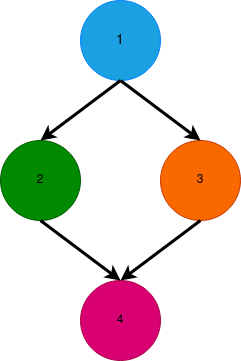
\includegraphics[scale=0.7]{Figures/reuse_example_graph.png}
\decoRule
\caption[reuseGraph]{Example of a graph with data reuse}
\label{fig:reuseGraph}
\end{figure}

Consider the computational graph of in figure \ref{fig:reuseGraph}. The graph clearly shows that
node 1's output will be reused as inputs to node 2 and 3. In a single SPM case,
we can see how the tensors would be mapped for each timestep. Clearly, the
leftover space of the SPM is what we can use as leftover pinning space between
operations. However, in the case of a multi-SPM architecture, this is not the
case as tensors cannot be split over different SPMs. To effectively navigate
the optimal mapping of pinned tensors, what SPM a tensor is pinned on greatly
affects the accumulated number of data transfers because of its effect on the
mapping of future tensors to an SPM. Once a tensor is pinned to a particular
SPM, mappings of inputs and outputs associated to other operations must be
remapped in accordance to the remaining capacity of all SPMs. This issue can be
compared to the bin-packing problem where the SPMs are bins and the tensors are
the items. Hence, for every possible mapping of a particular tensor to a SPM,
there exists new mapping for all other tensors that will exist for that
particular operation and future operations relative to the position of the
pinned tensor. The combinatorial explosion of possible mappings of tensors,
how long each one is mapped for, and where they are mapped is a search space
that grows with the depth of the deep learning model. An example of 
an un-optimal pinning strategy placing inputs and outputs without full consideration
of all future tensor placement combinations is shown in figure \ref{fig:pin_naive}.
In the figure, we can see that even though some tensors are able to be pinned,
there is unnecessary wasted space in some of the operations as well as other tensors
being written back and reloaded. Figure \ref{fig:pin_optimal} shows how a different
combination of tensor placements yields more reuse and less write backs to main
memory.

Notably, the single SPM case does not involve the concern of the exact location for
pinning a tensor. Rather, the decision making process in such a case is guided
solely by a tesnor's relative cost, its size, and the degree of overlap it has
with other tensors in terms of liveness. These factors shape how a pinned
tensor could influence future pinning opportunities for other tensors.
Due to these new considerations, simply porting the OnSRAM greedy algorithm 
leads to inefficient results since only a single scratchpad in the DLA can
be used for pinning.

Rather than porting the OnSRAM approach; a naively greedy approach in the
context of multiple SPMs has also been considered, i.e., initially pinning an
item to whatever SPM has the most space and remapping the inputs and outputs
accordingly. This process involves pinning outputs of every operation and
evicting the tensors when the pinned tensor cannot accommodate all other
necessary tensors for an operation, or when the output of the present operation
is of higher importance. The initial decision of selecting an SPM to pin an
item, which depends on the primary remapping of inputs and outputs around a
pinned tensor, can considerably influence the pinnability of future items. This
might, in certain instances, lead to the unpinned state of items immediately
prior to their reuse.

In such an approach, the system may not adequately identify opportunities for
reuse, leading to unpredictable decision-making and near-suboptimal results.
This limitation persists, albeit in a reduced form, even when the size of the
SPMs are increased. Therefore, to devise an algorithm that meticulously analyzes
possible decisions and maps tensors in a manner that effectively encourages
reuse, one could implement techniques such as graph coloring or ILP, which are
similar to the methods used in solving the pseudo-register SPM register
allocation problem.

Choosing an optimal pinning strategy to minimize the amount of data transfers
within this search space is the goal of this work.


\begin{figure}[th]
\centering
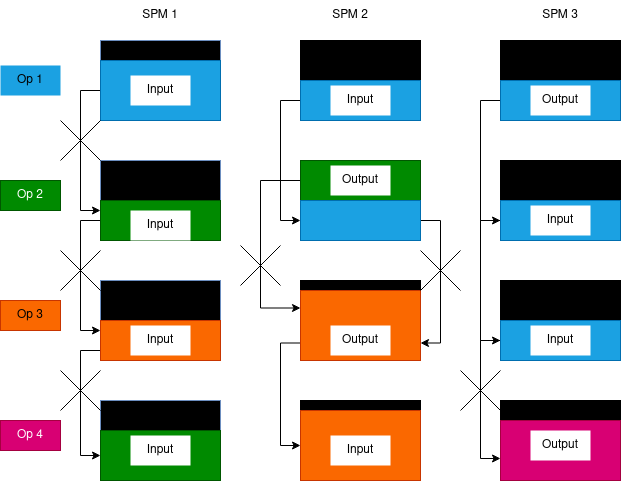
\includegraphics[scale=0.7]{Figures/reuse_example_pin_map_fail_1.png}
\decoRule
\caption[pin_naive]{Example of a un-optimal pinning strategy. Arrows
denote being pinned to the SPM and the crosses denote
an SPM being evicted due to capacity constraints.
Black denotes unused memory.}
\label{fig:pin_naive}
\end{figure}


\begin{figure}[th]
\centering
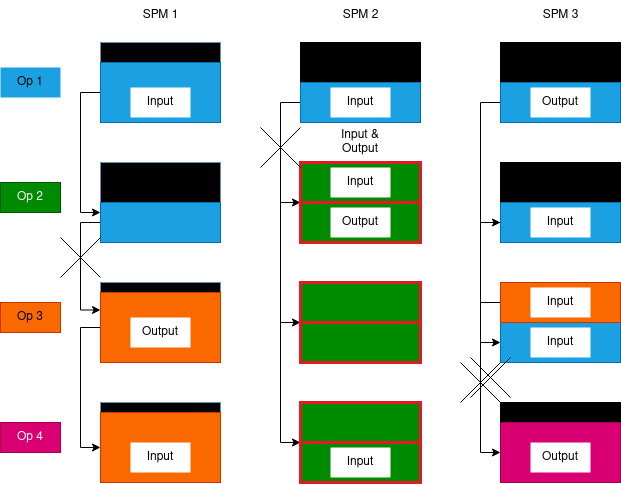
\includegraphics[scale=0.7]{Figures/reuse_example_pin_all.png}
\decoRule
\caption[pin_optimal]{Example of an optimal pinning strategy. Arrows
denote being pinned to the SPM and the crosses denote
an SPM being evicted due to capacity constraints. Red borders signify
distinction between different tensors created from the same operation.
Black denotes unused memory.}
\label{fig:pin_optimal}
\end{figure}
% we do everything in the 3 spm case
% goal is to mitigate data transfers between SPMs and main memory
% In order to analyze the possible mapping

\subsection{ILP based Multi-Scratchpad Allocation Strategy}
In order to analyze the search space and create a pin mapping for all tensors
such that the number of data transfers between SPMs and main memory on an
inter-node graph level are minimized, we propose an ILP model to create an
optimal strategy for a multi-scratchpad architecture.

To do this we first take an optimized computational graph and create a final
schedule of operators that will be ran. Using this schedule of operators, we
then aggregate all tensors that are used in the DNN. Each input and output
tensor is annotated with the operator from which it was created and all
operators that require it as a dependency. All tensor sizes, number of SPMs,
and the size of the SPMs are gathered as well. Using this information an
initial naive mapping scheme can be created where all inputs and outputs are
mapped to a designated input SPM and output SPM. All outputs are assumed to be
saved back to memory and reloaded when needed. We then use the initial mapping
as an input into the ILP solver to realize the optimal strategy.
